\documentclass{article}
\usepackage[utf8]{inputenc}
\usepackage[english]{babel}
\usepackage[style=numeric,sorting=ynt]{biblatex}
\usepackage[]{graphicx} % standard image package
\usepackage{svg} % include svg images
\usepackage{amsmath} % standard math package
\usepackage{float} % allow in place anchoring of images
\usepackage{multirow} % create nice tables
\usepackage{hyperref} % make links clickable

% Set up packages
\graphicspath{{../images/},{../images/movie_por0_stre6/},{../images/movie_por50_stre6/},{../images/movie_por50_stre3/},{../images/movie_por50_stre3_ang45/}}
\addbibresource{MasterThesis_References.bib}

% Commands
%\newcommand{\vec}{\boldsymbol}

% Metadata
\title{Smoothed Particle Hydrodynamics Simulations for Asteroid Deflection}
\author{Maximilian Rutz}
\date{}

%%%%%%%%%%%%%%%%%
% END OF PREAMBLE
%%%%%%%%%%%%%%%%%

\begin{document}

% Front page
\maketitle
\begin{abstract}
   Fragen:\\
- Wie viele gedruckte Exemplare?
- Abstract und Introduction?
\end{abstract}

% Contents page
\newpage
\tableofcontents

% Body
\newpage
\section{Introduction}
\begin{figure}[H]
    \centering
    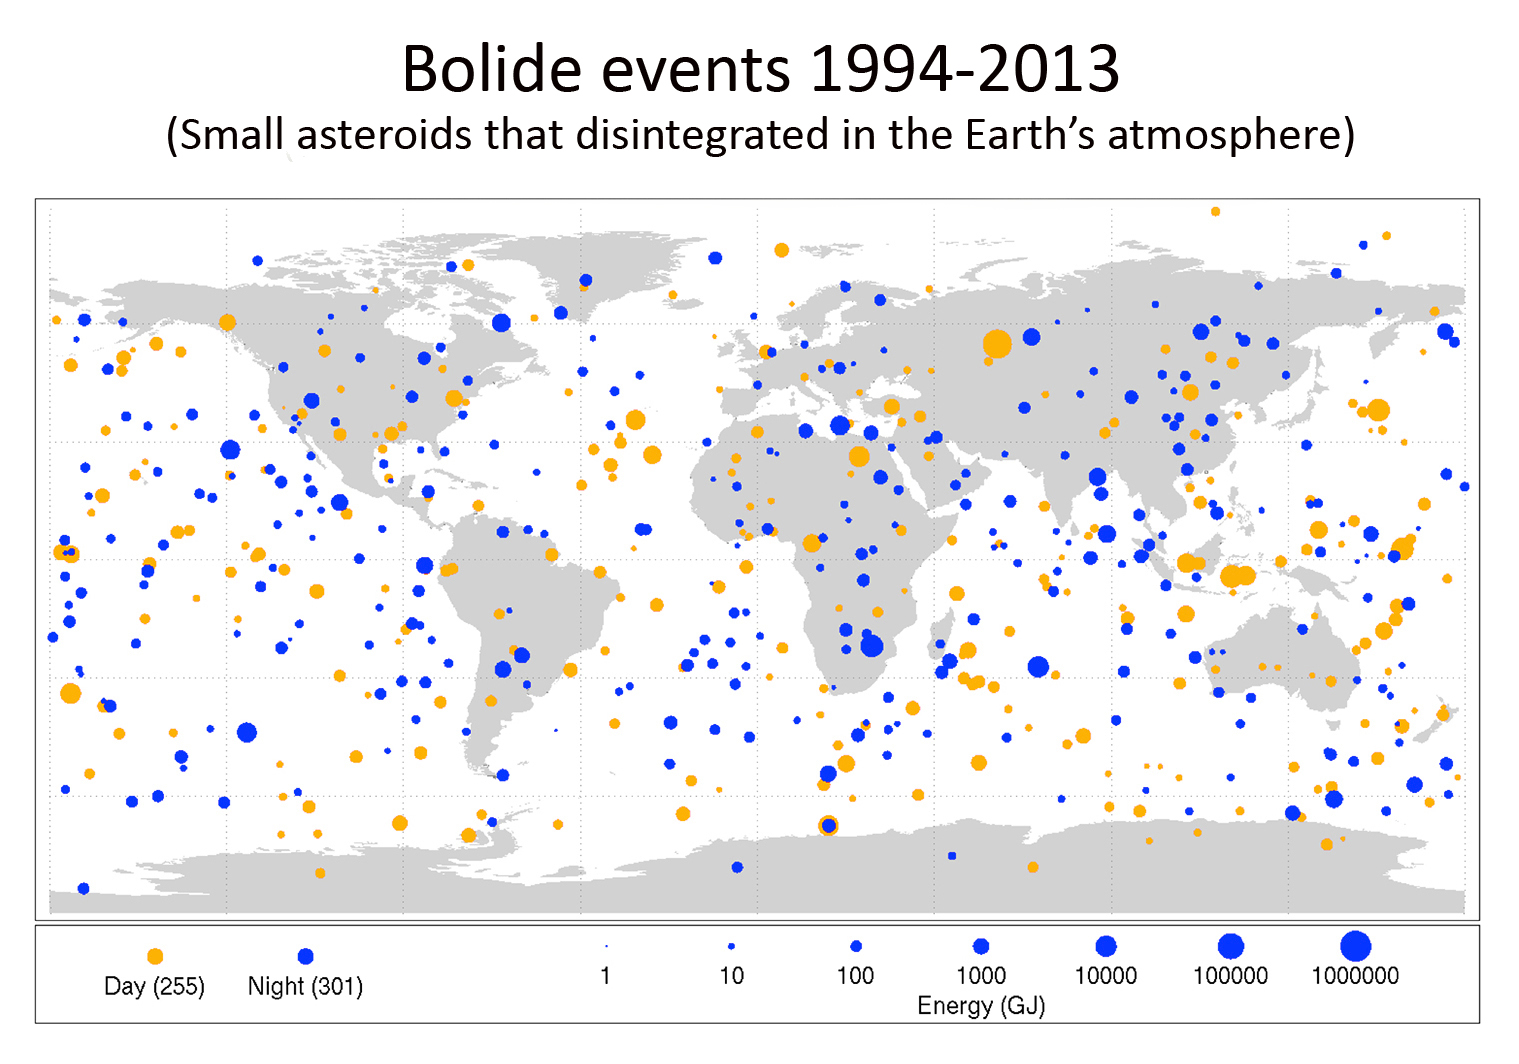
\includegraphics[width=\textwidth]{past_impacts.jpg}
    \caption{Past impacts \cite{wiki:past_impacts}}
    \label{fig:past_impacts}
\end{figure}


- test case for p-alpha porosity and pressure dependent yield strength

- Raducan \cite{Raducan_2019_strength} grid based 2d sims
- Stickle \cite{Stickle_2017}
\newpage
\section{Theory}
- Equations from Geophysics/Continuum Mechanics and High velocity impact physics that are needed to model the Impact

- all parameters that appear in the table of the Numerics section should be explained

\subsection{Conservation equations}
- mass
- momentum
- energy

\subsection{Constitutive equations}
- time evolution of deviatoric stress tensor


\subsection{Equation of State}
- Tillotson equation of state \cite{Tillotson_1962}

\subsection{Porosity model}
There are different ways in which porosity can be modeled depending on the pore size. Depending on the simulation, macro porosity with pore sizes above the resolution of the simulation can be accounted for in the initial conditions. This however becomes impossible for granular material with sub-resolution sized grains and pores.

Microporosity models porosity as an additional material property and can be applied independently of the resolution.


In these simulations, a microporosity p-$\alpha$ model as outlined in \cite{Jutzi_2008} is used. The distention $\alpha \in [1,\inf)$ relates the current density $\rho$ to the solid density $\rho_s$ which is reached if the material is fully compressed. For a non-porous material $\alpha$ equals one.

\begin{equation}
    \alpha \equiv \frac{\rho_s}{\rho}
\end{equation}

Often the porosity $\phi$ is used instead of the distention $\alpha$. They relate by

\begin{equation}
    \phi = 1 - \frac{1}{\alpha}
\end{equation}

- Quadratic crush curve

\subsection{Fragmentation model}
- fracture of brittle material
- Weibull distribution

\subsection{Strength model}
- elastic and plastic regimes
- von Mises strength
- pressure dependent yield strength

- ideas in \cite{Collins_2004}
- implementation in \cite{Jutzi_2015}
\newpage
\section{Numerical Setup}
\subsection{Miluphcuda SPH code}
Miluphcuda is a smoothed particle hydrodynamics code that has been developed over several years at the University of Tuebingen by Christoph Schaefer and others. Its general use is well documented in \cite{Schaefer_2016}.


\subsection{Initial conditions}
- Target basalt halfsphere
- Impactor aluminium sphere
- resolution bound to variable smoothing length
- Uniform macro structure but random micro structure to avoid
- seagen \cite{github:SEAGen} used to create initial conditions

\begin{figure}[H]
    \centering
    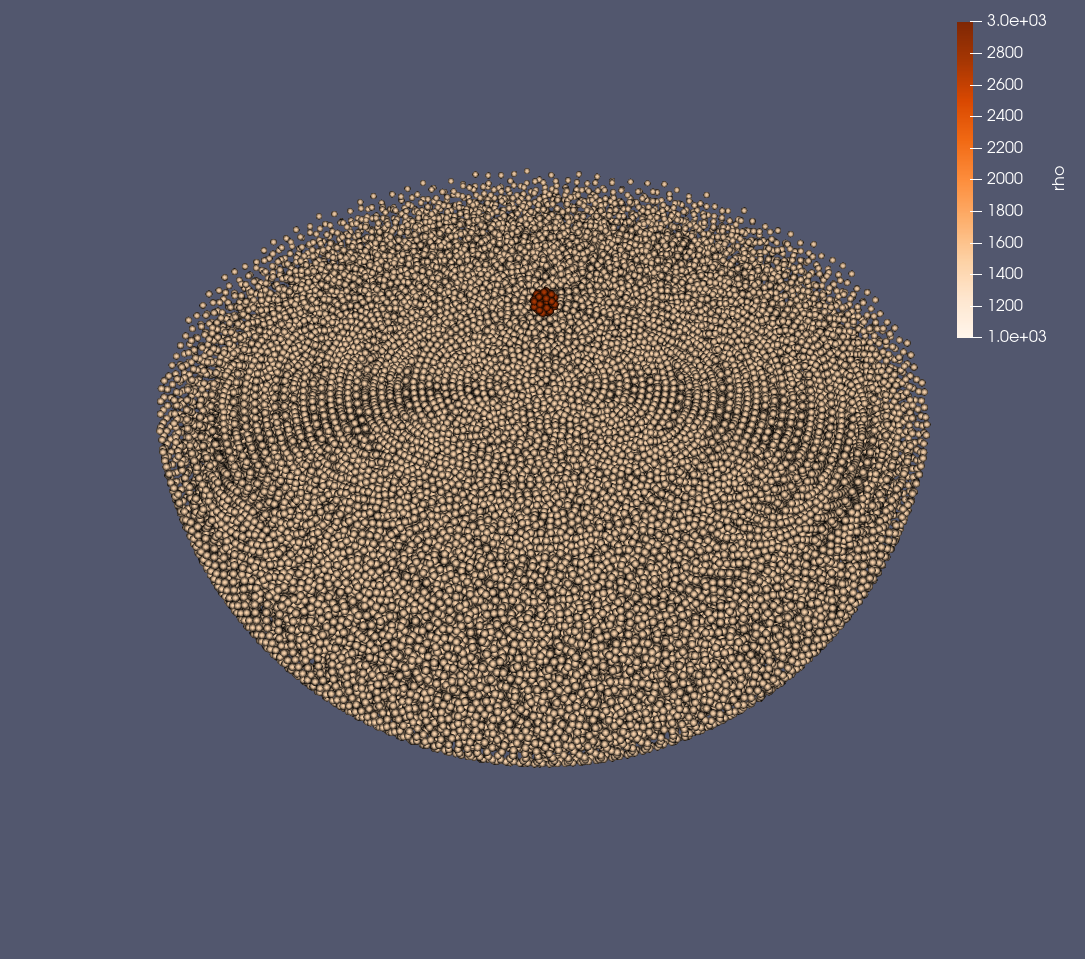
\includegraphics[width=\textwidth]{impact_start.png}
    \caption{start of simulation}
    \label{fig:impact_start}
\end{figure}

\begin{figure}[H]
    \centering
    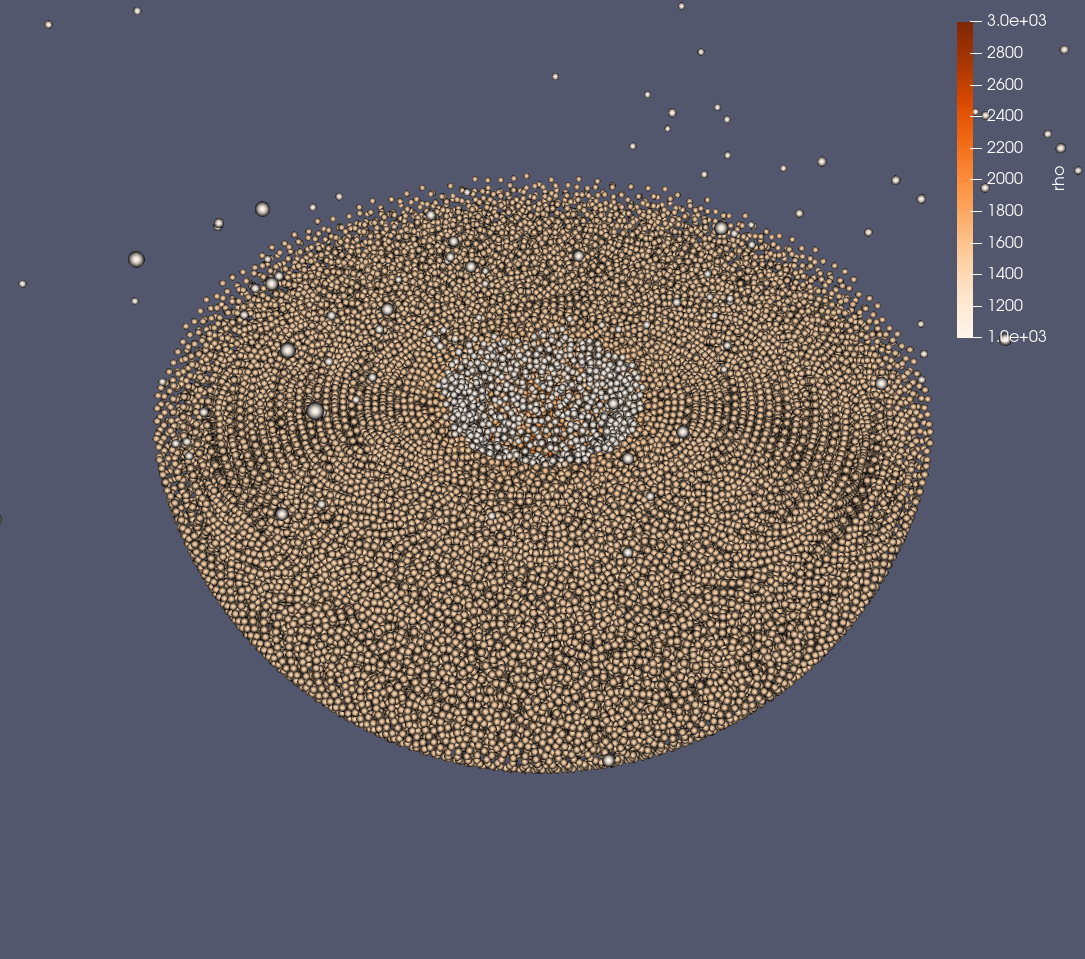
\includegraphics[width=\textwidth]{impact_end.png}
    \caption{end of simulation}
    \label{fig:impact_end}
\end{figure}

\subsection{Material parameters}

\begin{table}
    \centering
    \begin{tabular}{ |l|l|l|l| }
        \hline
        \multicolumn{2}{|c|}{}                & Target                  & Projectile                                                          \\
        \hline
        \multirow{10}{*}{Tillotson EOS}       & $\rho_0$                & 2.86 $\cdot 10^3 g\cdot cm^{-3}$ & 2.70 $\cdot 10^3 g\cdot cm^{-3}$ \\
                                              & $A_T$                   & 2.67 $\cdot 10^{10}$ Pa          & 7.52 $\cdot 10^{10}$ Pa          \\
                                              & $B_T$                   & 2.67 $\cdot 10^{10}$ Pa          & 6.50 $\cdot 10^{10}$ Pa          \\
                                              & $E_0$                   & 4.87 $\cdot 10^8$ J              & 5.00 $\cdot 10^6$ J              \\
                                              & $E_{iv}$                & 4.72 $\cdot 10^6$ J              & 3.00 $\cdot 10^6$ J              \\
                                              & $E_{cv}$                & 1.82 $\cdot 10^7$ J              & 1.39 $\cdot 10^7$ J              \\
                                              & $a_T$                   & 0.5                              & 0.5                              \\
                                              & $b_T$                   & 1.5                              & 1.63                             \\
                                              & $\alpha_T$              & 5.0                              & 5.0                              \\
                                              & $\beta_T$               & 5.0                              & 5.0                              \\ \hline
        \multirow{7}{*}{Porosity}             & $\alpha_0$              & \textbf{varying}                 & not porous                       \\
                                              & $p_{elastic}$           & 1.0 $\cdot 10^6$ Pa              & not porous                       \\
                                              & $p_{transition}$        & 6.8 $\cdot 10^7$ Pa              & not porous                       \\
                                              & $p_{compacted}$         & 2.13 $\cdot 10^8$ Pa             & not porous                       \\
                                              & $\alpha_e$              & 4.64                             & not porous                       \\
                                              & $\alpha_t$              & 1.90                             & not porous                       \\
                                              & $c_s$                   & 100.0 $m\cdot s^{-1}$            & not porous                       \\ \hline
        \multirow{6}{*}{Strength}             & cohesive strength $Y_c$ & \textbf{varying}                 & 1.0 $\cdot 10^9$ Pa              \\
                                              & $\alpha$                & 0.982793 rad                     & 0 rad                            \\
                                              & $\alpha_{damaged}$      & 0.540419 rad                     & 0 rad                            \\
                                              & shear modulus $\mu$     & 2.27 $\cdot 10^{10}$ Pa          & 2.69 $\cdot 10^{10}$ Pa          \\
                                              & bulk modulus $K_0$      & 2.67 $\cdot 10^{10}$ Pa          & 5.23 $\cdot 10^{10}$ Pa          \\
                                              & yield stress $Y_0$      & 3.5 $\cdot 10^9$ Pa              & 2.76 $\cdot 10^8$ Pa             \\ \hline
        \multirow{2}{*}{Weibull}              & M                       & 16                               & no damage                        \\
                                              & K                       & 1.0 $\cdot 10^{61}$              & no damage                        \\ \hline
        \multirow{2}{*}{Artificial viscosity} & $\alpha$                & 1.0                              & 1.0                              \\
                                              & $\beta$                 & 2.0                              & 2.0                              \\ \hline
        \hline
    \end{tabular}
    \caption{Material parameters for basalt target and aluminium Impactor}
    \label{fig:material_parameters}
\end{table}

- variable smoothing length min 0.1 bis max 10.0
- rholimit 0.95
\newpage
\section{Results}
The simulations were run with porosities of 0\%, 17\%, 33\% and 50\% and cohesive strengths of 1kPa, 10kPa, 100kPa and 1MPa under impact angles of 0 and 45 degrees. This yields 32 simulations in total.

\subsection{Cratering}
- qualitative analysis

- head on
\begin{figure}[H]
   \centering
   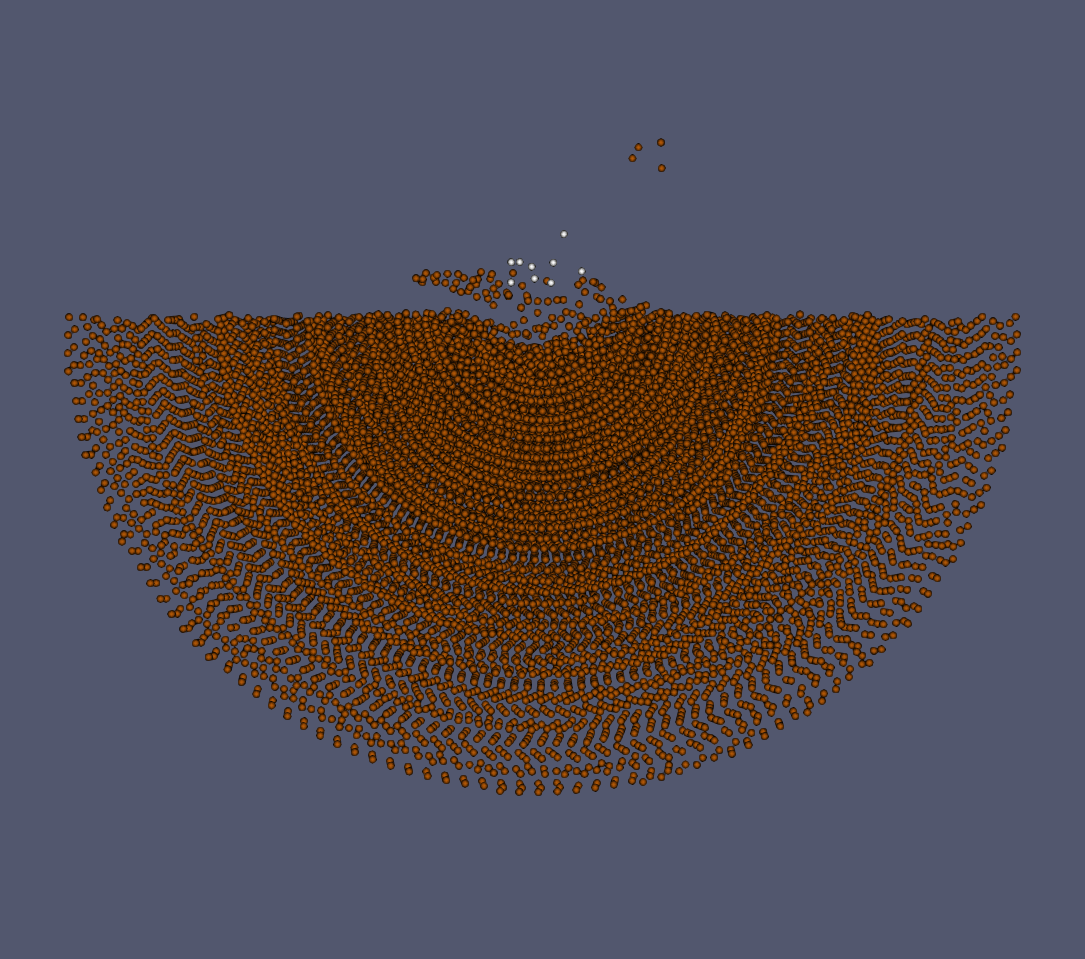
\includegraphics[width=\textwidth]{crater_por0_stre6.png}
   \caption{No porosity (0\%), high strength (Y=1MPa)}
   \label{fig:crater1}
\end{figure}


\begin{figure}[H]
   \centering
   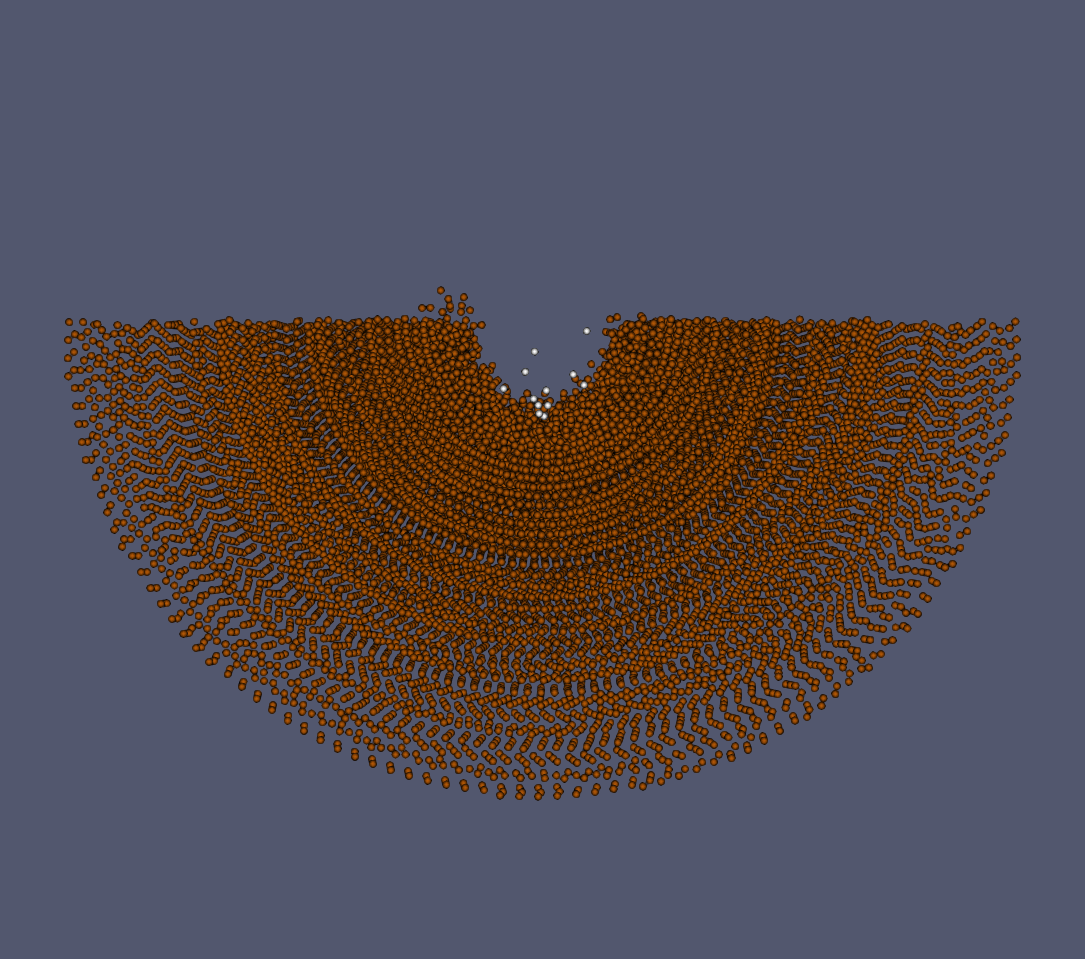
\includegraphics[width=\textwidth]{crater_por50_stre6.png}
   \caption{High porosity (50\%), high strength (Y=1MPa)}
   \label{fig:crater2}
\end{figure}

\begin{figure}[H]
   \centering
   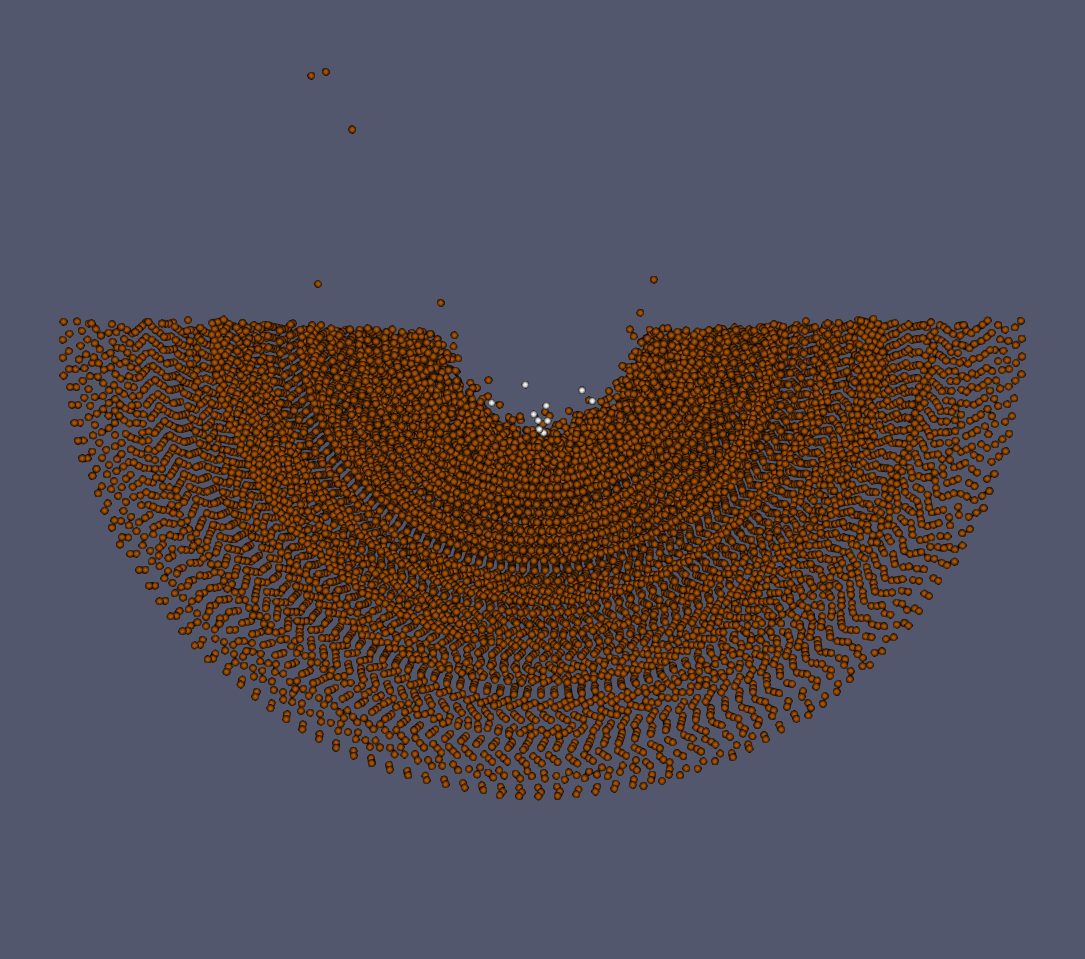
\includegraphics[width=\textwidth]{crater_por50_stre3.png}
   \caption{High porosity (50\%), low strength (Y=1kPa)}
   \label{fig:crater3}
\end{figure}

- 45 degrees
\begin{figure}[H]
   \centering
   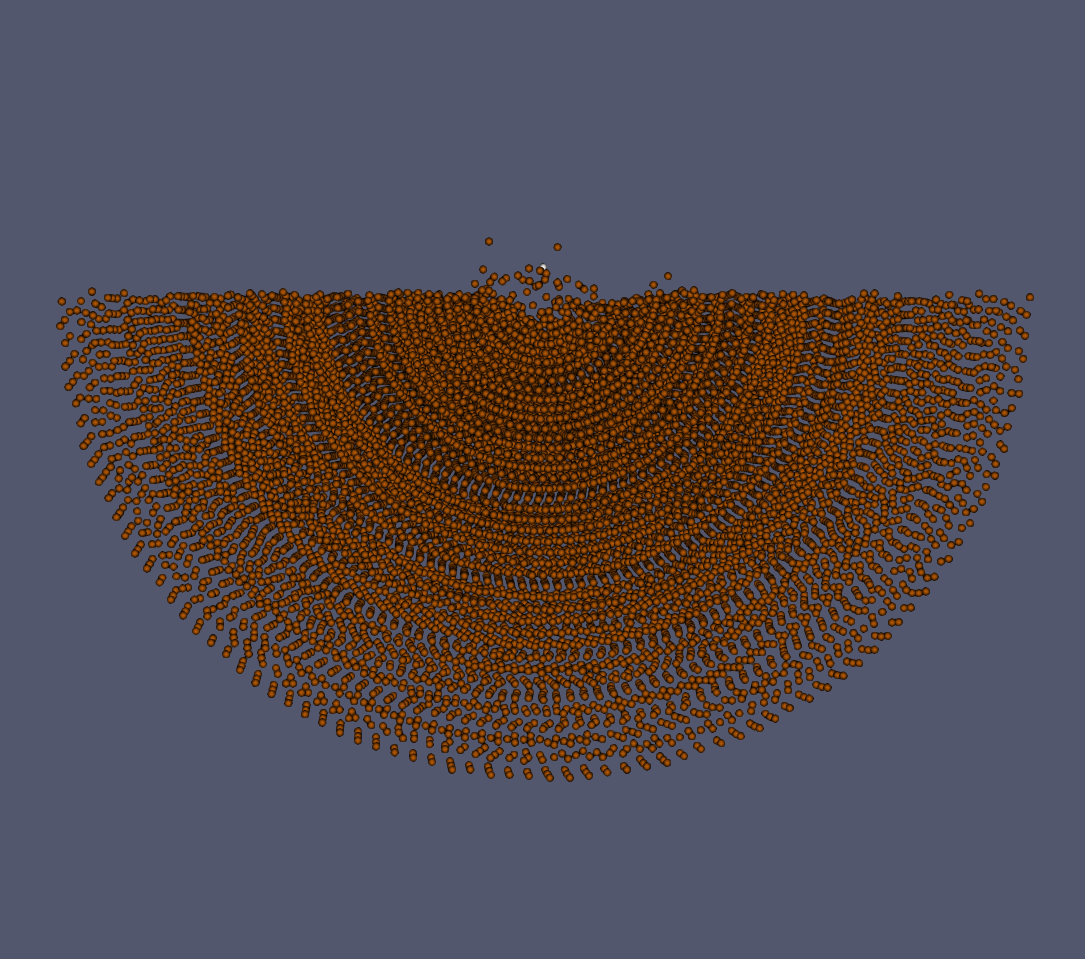
\includegraphics[width=\textwidth]{crater_por0_stre6_ang45.png}
   \caption{No porosity (0\%), high strength (Y=1MPa), 45 degree angle}
   \label{fig:crater4}
\end{figure}


\begin{figure}[H]
   \centering
   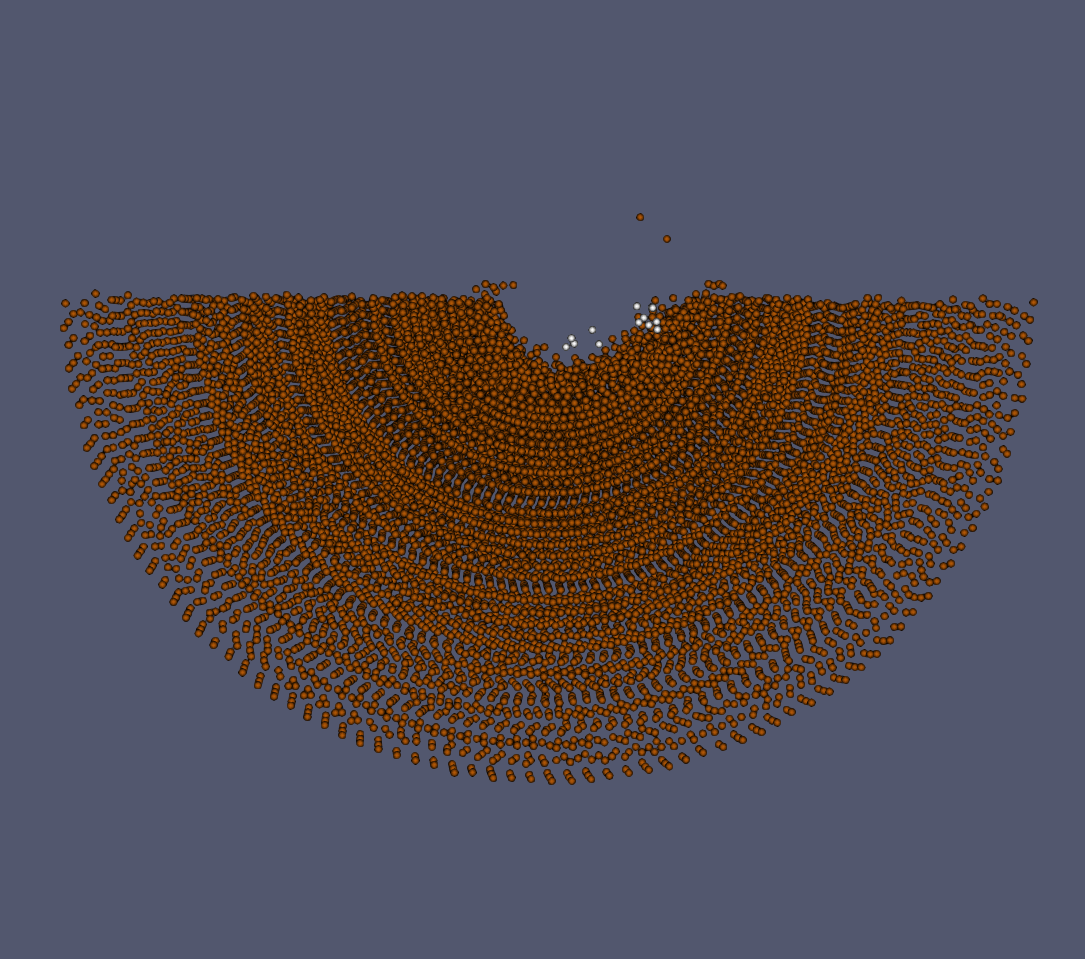
\includegraphics[width=\textwidth]{crater_por50_stre6_ang45.png}
   \caption{High porosity (50\%), high strength (Y=1MPa), 45 degree angle}
   \label{fig:crater5}
\end{figure}

\begin{figure}[H]
   \centering
   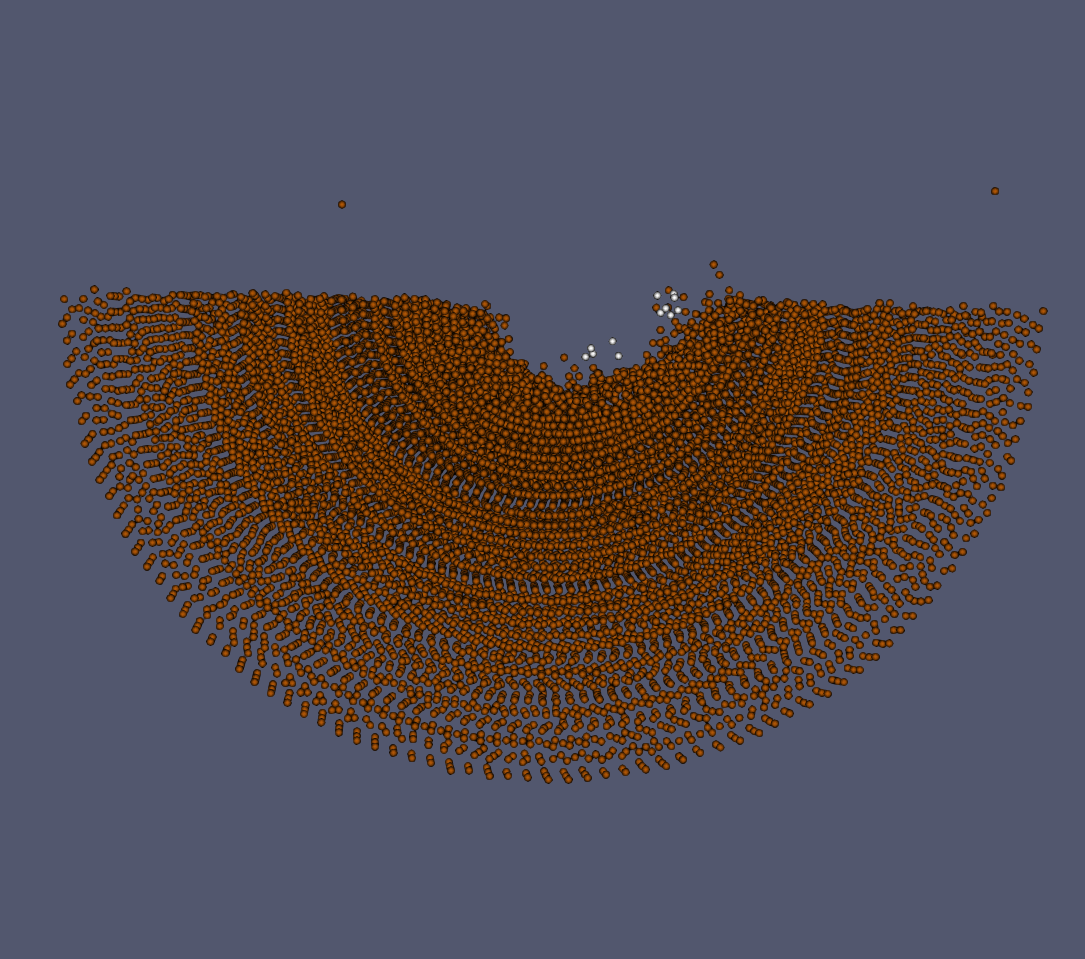
\includegraphics[width=\textwidth]{crater_por50_stre3_ang45.png}
   \caption{High porosity (50\%), low strength (Y=1kPa), 45 degree angle}
   \label{fig:crater6}
\end{figure}

\subsection{Damage}

\begin{figure}[H]
   \centering
   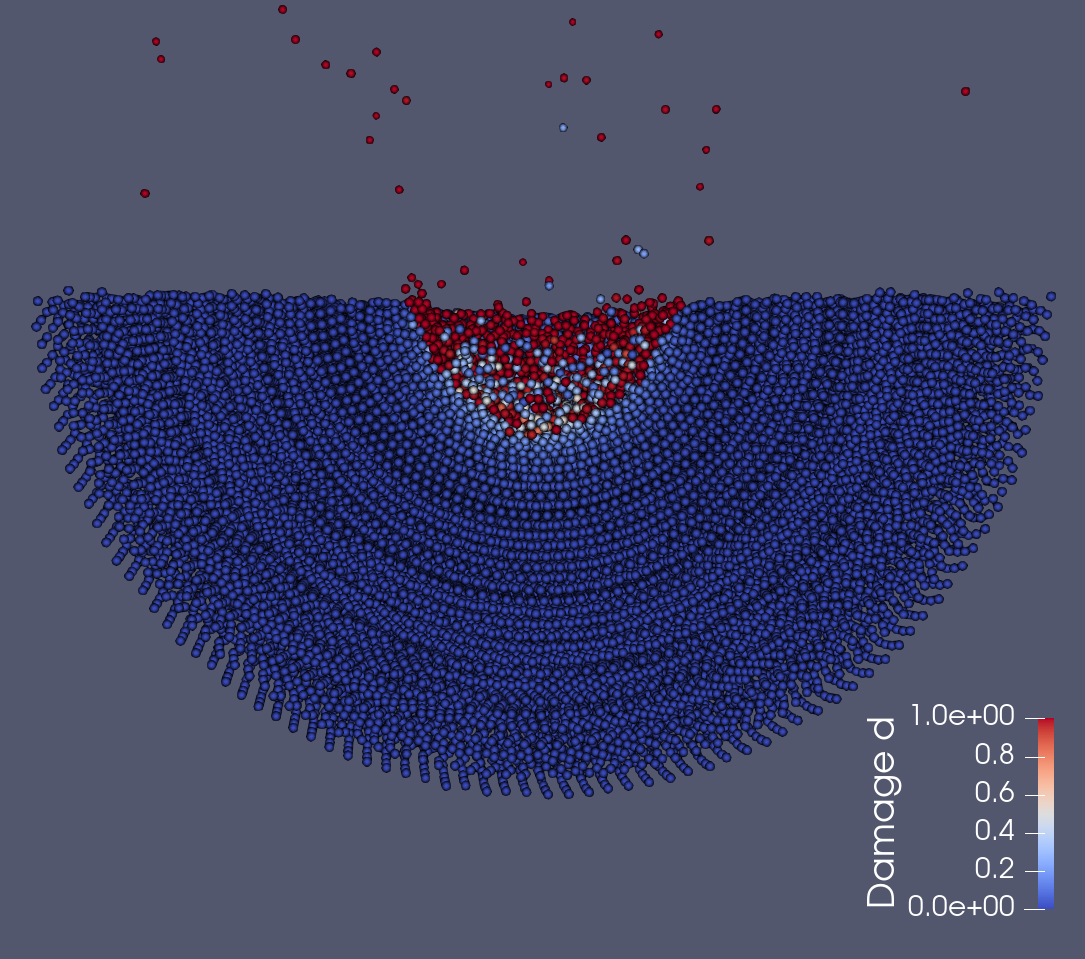
\includegraphics[width=\textwidth]{damage_por50_stre3.png}
   \caption{Damage high porosity (50\%), low strength (Y=1kPa)angle}
   \label{fig:crater6}
\end{figure}

\begin{figure}[H]
   \centering
   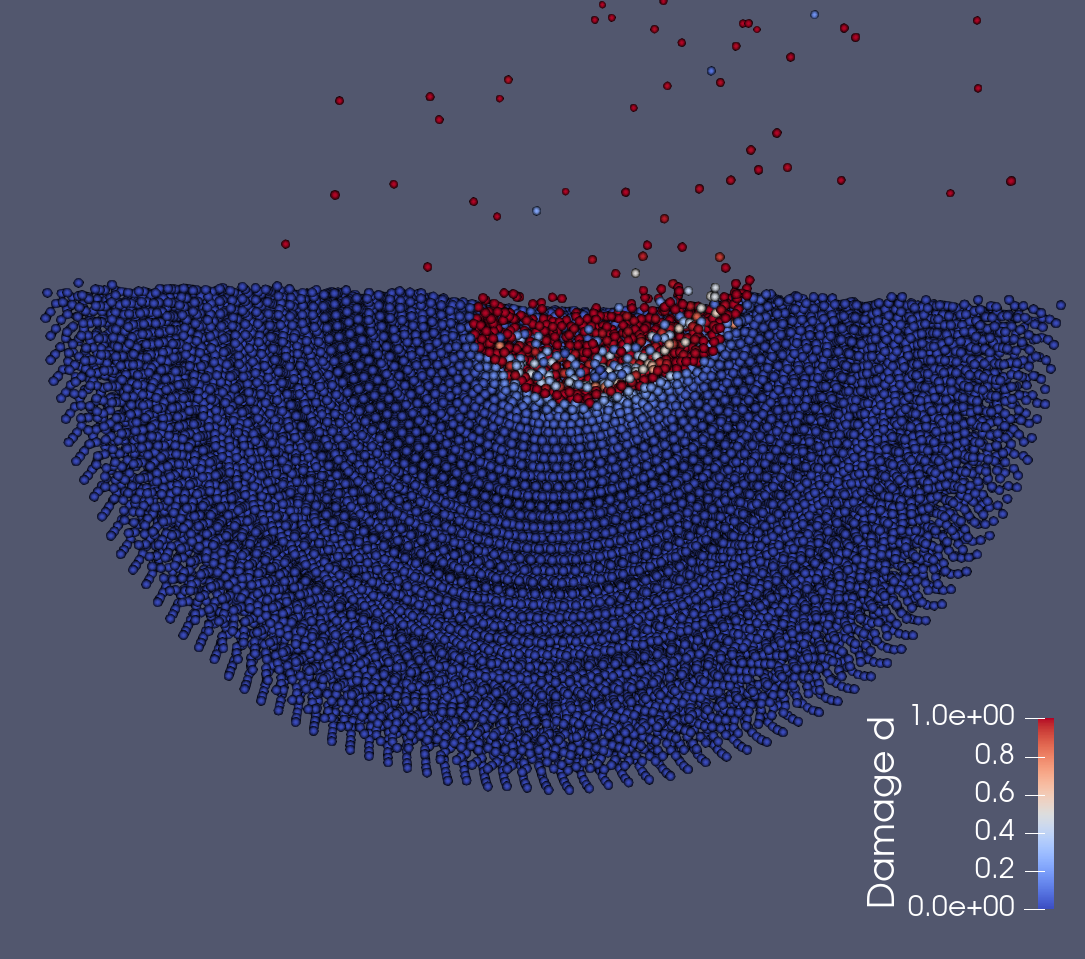
\includegraphics[width=\textwidth]{damage_por50_stre3_ang45.png}
   \caption{Damage high porosity (50\%), low strength (Y=1kPa), 45 degree angle}
   \label{fig:crater6}
\end{figure}

\subsection{Distention}

\begin{figure}[H]
   \centering
   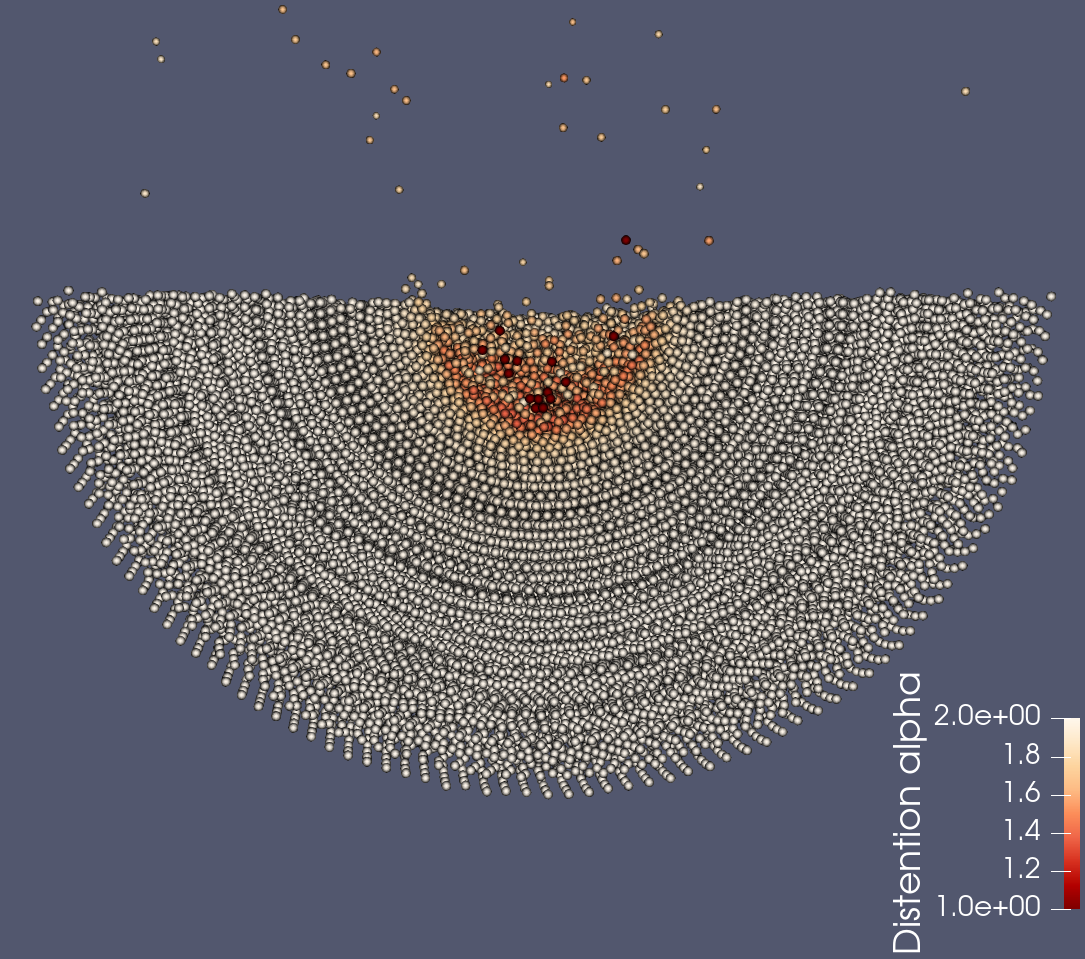
\includegraphics[width=\textwidth]{distention_por50_stre3.png}
   \caption{Distention high porosity (50\%), low strength (Y=1kPa)angle}
   \label{fig:crater6}
\end{figure}

\begin{figure}[H]
   \centering
   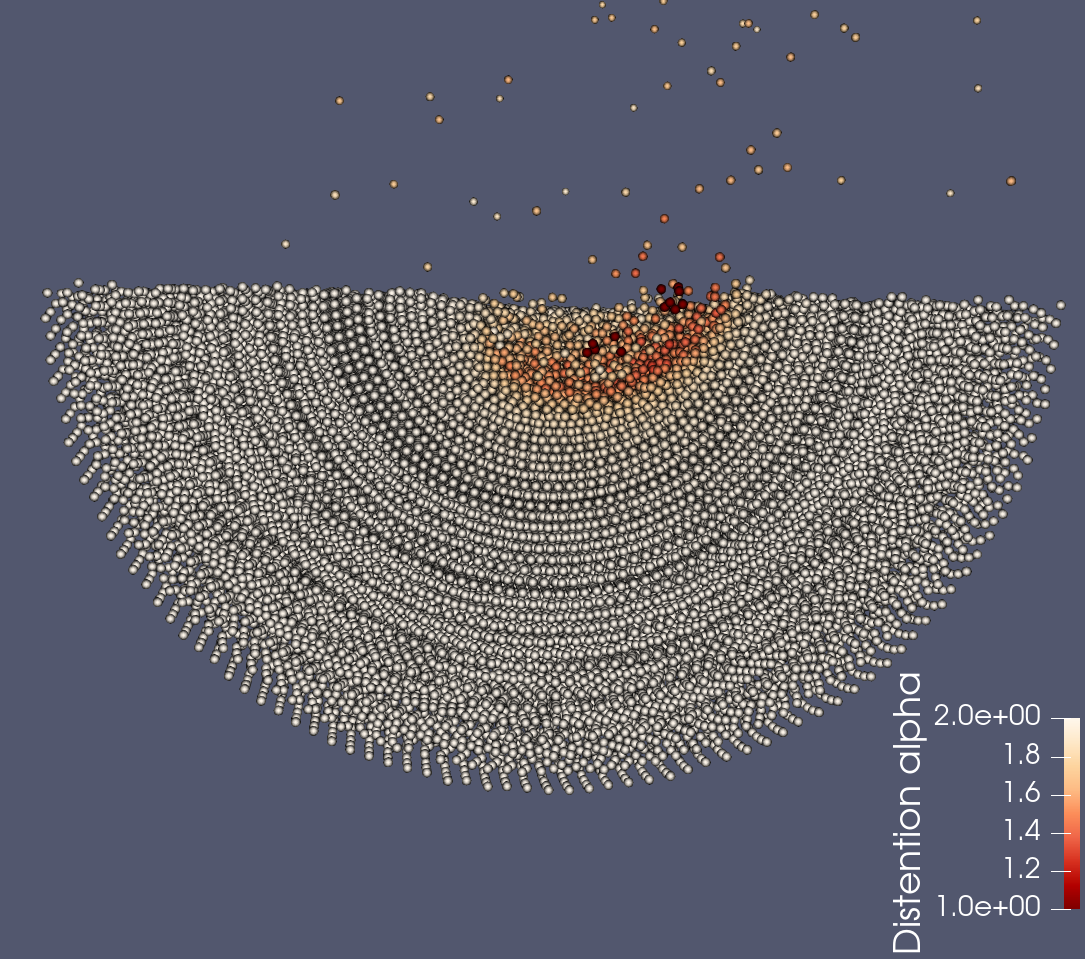
\includegraphics[width=\textwidth]{distention_por50_stre3_ang45.png}
   \caption{Distention high porosity (50\%), low strength (Y=1kPa), 45 degree angle}
   \label{fig:crater6}
\end{figure}

\subsection{Beta factor}
- explanation of beta factor

\begin{figure}[H]
   \centering
   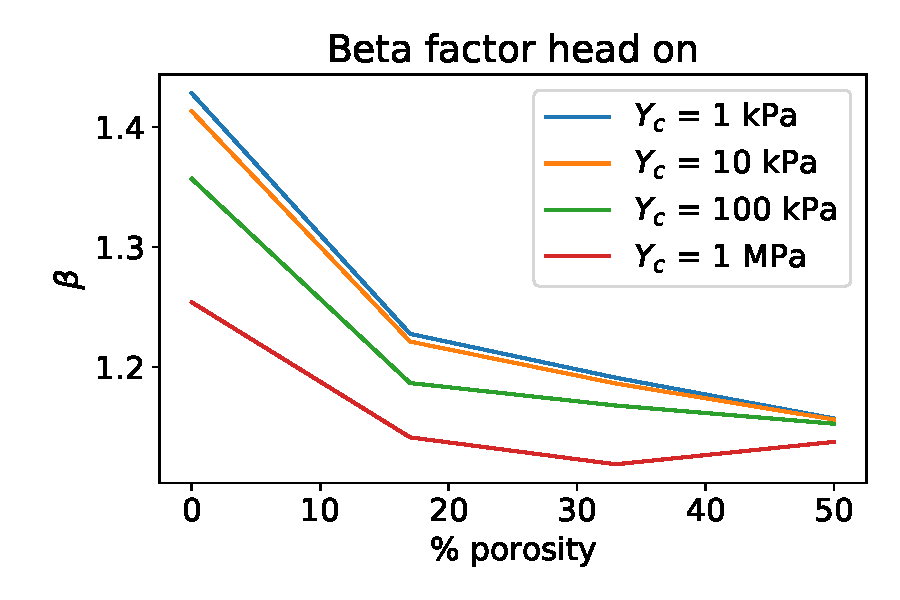
\includegraphics[width=\textwidth]{beta_results_ang0.pdf}
   \caption{beta factor}
   \label{fig:beta_factor_0}
\end{figure}

\begin{figure}[H]
   \centering
   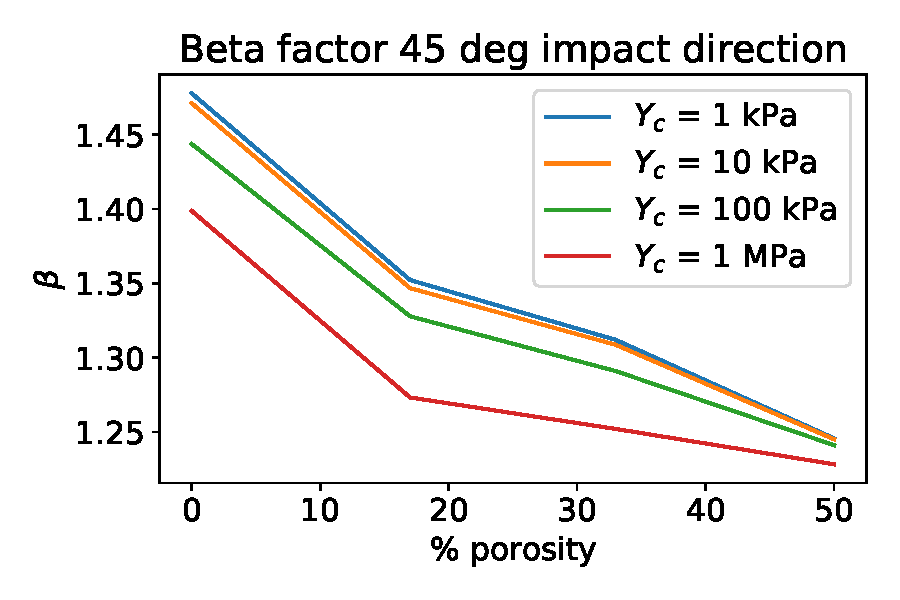
\includegraphics[width=\textwidth]{beta_results_ang45_impact.pdf}
   \caption{beta factor in impact direction}
   \label{fig:beta_factor_45_impact}
\end{figure}

\begin{figure}[H]
   \centering
   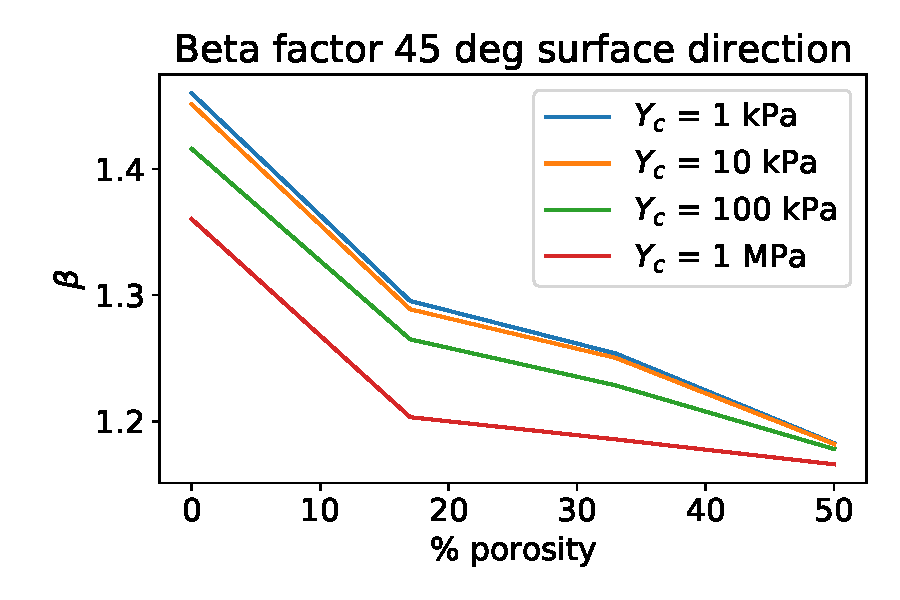
\includegraphics[width=\textwidth]{beta_results_ang45_surface.pdf}
   \caption{beta factor perpendicular to surface}
   \label{fig:beta_factor_45_surface}
\end{figure}

- only particles with positive velocity along impact direction above escape velocity
\begin{equation}
   v_{esc} = \sqrt{\left(\dfrac{2GM}{r_i}\right)}
\end{equation}
where $M = \frac{4}{3}\pi R^3 \rho_{asteroid}$ is the estimated mass of asteroid with R = 75m and $\rho{asteroid}$ = 2.8$\frac{g}{cm^3}$ and $r_i$ distance of sph particle from center of estimated asteroid sphere
- few particles (with highest velocities so the ones that are far away) account for most of the momentum

\begin{figure}[H]
   \centering
   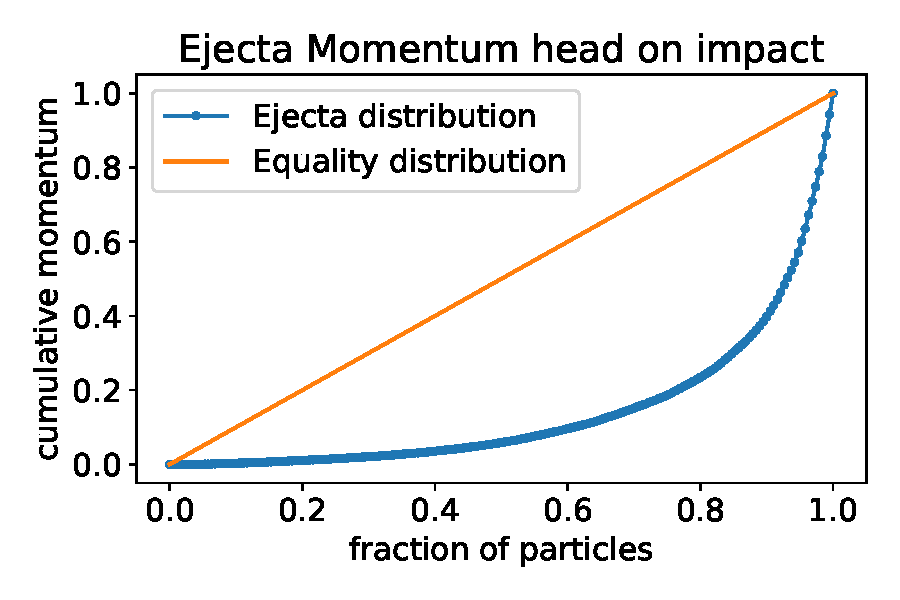
\includegraphics[width=\textwidth]{beta_lorenz_ang0.pdf}
   \caption{Lorenz curve for momentum distribution head on}
   \label{fig:beta_factor_lorenz_0}
\end{figure}

\begin{figure}[H]
   \centering
   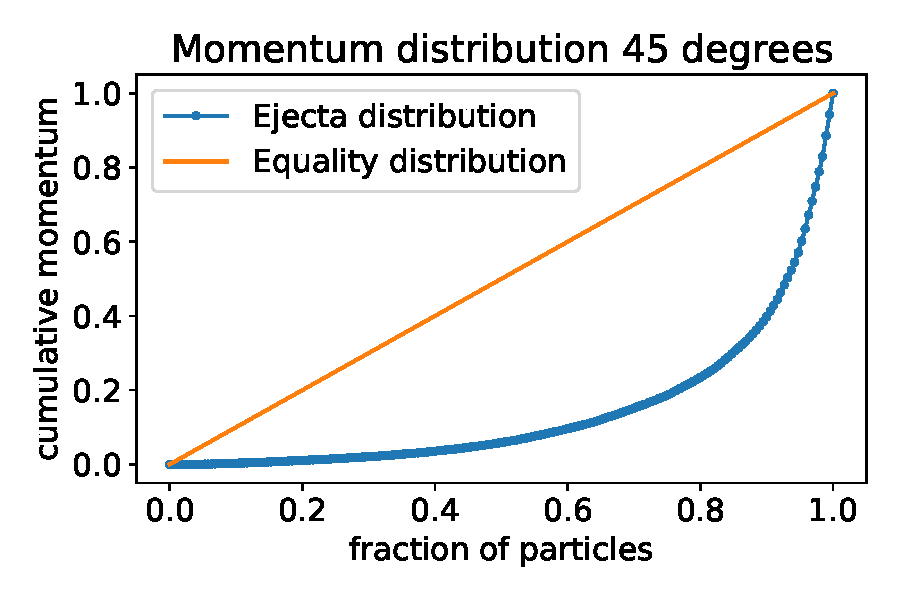
\includegraphics[width=\textwidth]{beta_lorenz_ang45.pdf}
   \caption{Lorenz curve for momentum distribution 45 degree}
   \label{fig:beta_factor_lorenz_45}
\end{figure}
\newpage
\section{Discussion}
- beta factor on the lower end
- upper limit beta < 2 because of momentum conservation??

% References
\newpage
\printbibliography

\end{document}